\documentclass{beamer}
\usepackage{graphicx}
\usepackage{paralist}
\usepackage{outlines}

\title{Colour Correction}
\author{Mendocino College - Digital Image Manipulation with Photoshop}
\titlegraphic{\vspace{-10mm}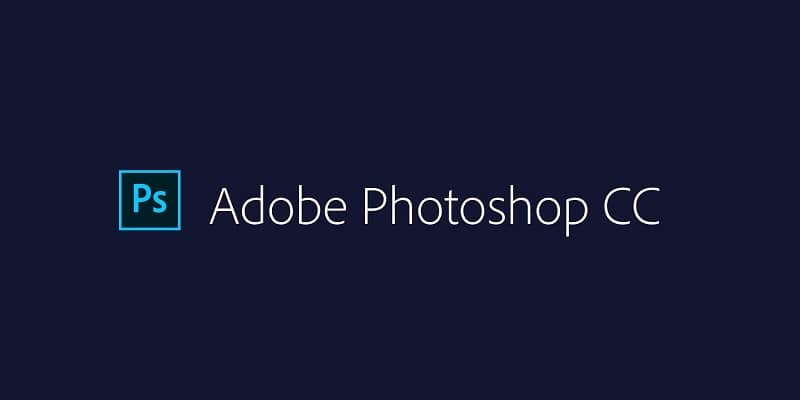
\includegraphics[width = .9\textwidth]{images/photoshop.jpg}} 
\date{\vspace{-5em}} 


\mode <presentation>
\usetheme{Warsaw}
\usecolortheme{default}

\setbeamerfont{footline}{size=\fontsize{5}{8}\selectfont}

\definecolor{darkred}{rgb}{20,0,0}
\definecolor{darkgreen}{RGB}{40,110,20}
\definecolor{darkpurple}{RGB}{30,0,30}
\definecolor{chardonnay}{RGB}{255, 255, 204}

\setbeamercolor*{palette primary}{fg=white, bg=darkgreen}


\begin{document}
	{
		\setbeamertemplate{footline}{} 
		\setbeamertemplate{headline}{} 
		\begin{frame}
			\vspace{-35pt}
			\maketitle
		\end{frame}
	}

	\section{Levels Adjustment Layer}
\subsection{Levels Adjustment Layer}		
\begin{frame}
	\frametitle{Levels Adjustment Layer}
	\begin{columns}
		\column{.7\textwidth}
		\begin{outline}
			\1  Used to correct the tonal range and color balance of an image by adjusting intensity levels of image shadows, midtones, and highlights. 
			\1 The Levels histogram is a visual guide for adjusting the image key tones.
			\1 Use to sliders to adjust the black point and white point.
			\2 The middle slider adjusts gamma (intensity, or midtones)
			\1 Use the eyedroppers next to the histogram to set the white/midtone/black points for your image.
		\end{outline}
		\column{.45\textwidth}
		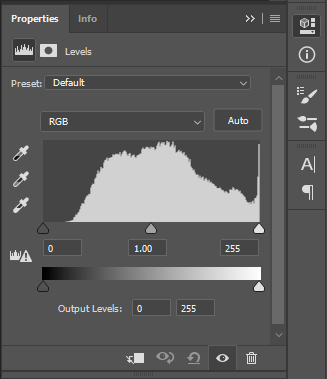
\includegraphics[width=1.0\textwidth]{images/levels.png}
	\end{columns}
\end{frame}

\subsection{Clipping}		
\begin{frame}
	\frametitle{Clipping}
		\begin{outline}
			\1  Clipping is when the pixels are completely washed out with no detail.
			\2 When shadows are clipped, the pixels are black, with no detail. 
			\2 When highlights are clipped, the pixels are white, with no detail.
			\1 You can preview clipping as you adjust black and white points by holding down the Alt key.
		\end{outline}
\end{frame}

		\section{Curves Adjustment Layer}
			\subsection{Curves Adjustment Layer}		
			\begin{frame}
				\frametitle{Curves Adjustment Layer}
				\begin{columns}
					\column{.75\textwidth}
					\begin{outline}
						\1 In the Curves adjustment, you adjust points throughout an image’s tonal range.
						\1 Initially, the image’s tonality is represented as a straight diagonal line on a graph.
						\1 The upper-right area of the graph represents the highlights 
						\2 The lower-left area represents the shadows. 
						\2 The horizontal axis of the graph represents the input levels (original image values) 
						\2 The vertical axis represents the output levels (new adjusted values)
						\1 The steeper sections of the curve represent areas of higher contrast 
						\2 While the flatter sections represent areas of lower contrast.
					\end{outline}
					\column{.4\textwidth}
					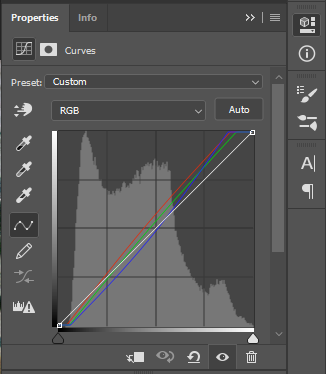
\includegraphics[width=1.0\textwidth]{images/Curves.png}
				\end{columns}
			\end{frame}
			
			\subsection{Masks}		
			\begin{frame}
				\frametitle{Masks}
				\begin{columns}
					\column{.65\textwidth}
					\begin{outline}
						\1 Curves (and Levels) are applied to your image as a mask.
						\1 This allows your edits to be non-destructive.
						\1 You are also able to control which part of the image is effected.
						\1 You can change the adjustment layers mask by double-clicking the mask in the layers panel.
						\2 From here, you can either select objects to apply your adjustment too
						\2 Or use the brush tool to "paint" the area's to be adjusted.
					\end{outline}
					\column{.5\textwidth}
					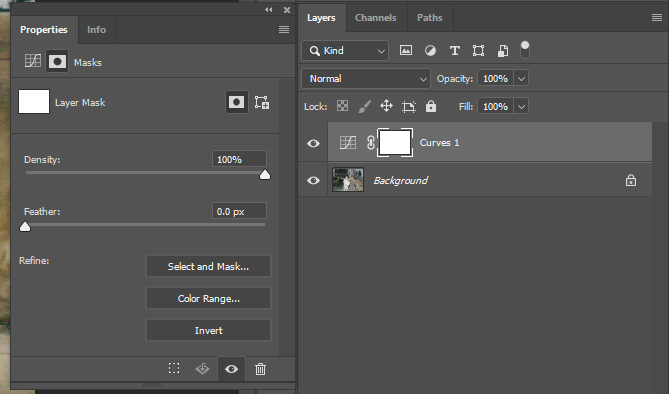
\includegraphics[width=1.0\textwidth]{images/curves mask.png}
				\end{columns}
			\end{frame}
			
			
			
			
		\section{Auto Correction Options}
			\subsection{Auto Correction Options}		
			\begin{frame}
				\frametitle{Auto Correction}
				\begin{outline}
					\1 Both Levels and Curves have very good built-in auto-correction options.
					\1 To find them, Open the properties panel for your Level (or Curves) adjustment layer.
					\2 Do this by double-clicking the layer thumbnail of the adjustment layer in the layers panel.
					\1 Then click the 4 stacked horizontal bars (under the x to close the panel).
					\1 Select "Auto Options..."
				\end{outline}
				\begin{center}
					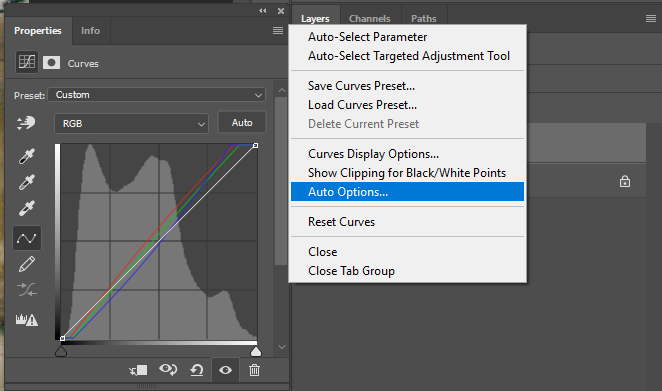
\includegraphics[width=0.65\textwidth]{images/auto correction.png}
				\end{center}
			\end{frame}		
		
					\begin{frame}
			\frametitle{Auto Correction Options}
				\begin{columns}
					\column{.65\textwidth}
					\begin{outline}
						\1 Here you have 4 different algorithms to utilize.
						\1 Each algorithm uses a different method to make corrections to your images colours and tone.
						\1 You can also adjust the algorithms by setting your own targets for shadows/midtones/highlights.
					\end{outline}
					\column{.55\textwidth}
					\begin{center}
						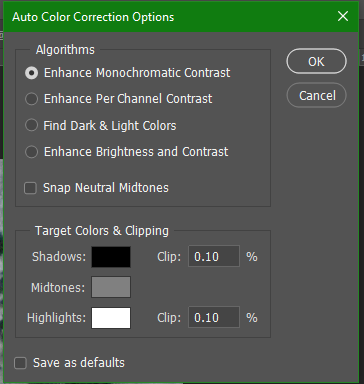
\includegraphics[width=0.9\textwidth]{images/auto correction options.png}
					\end{center}
				\end{columns}

		\end{frame}		
		
		\section{Adobe Bridge and Camera Raw}
			\subsection{Adobe Bridge and Camera Raw}				
				\begin{frame}
					\frametitle{Adobe Bridge}
					\begin{outline}
						\1 To access Camera Raw, you must use Adobe Bridge.
						\1 Open Adobe Bridge
						\2 Navigate to your image
						\2 Right-click the image
						\2 Select "Open in Camera Raw..."
					\end{outline}
				\begin{center}
					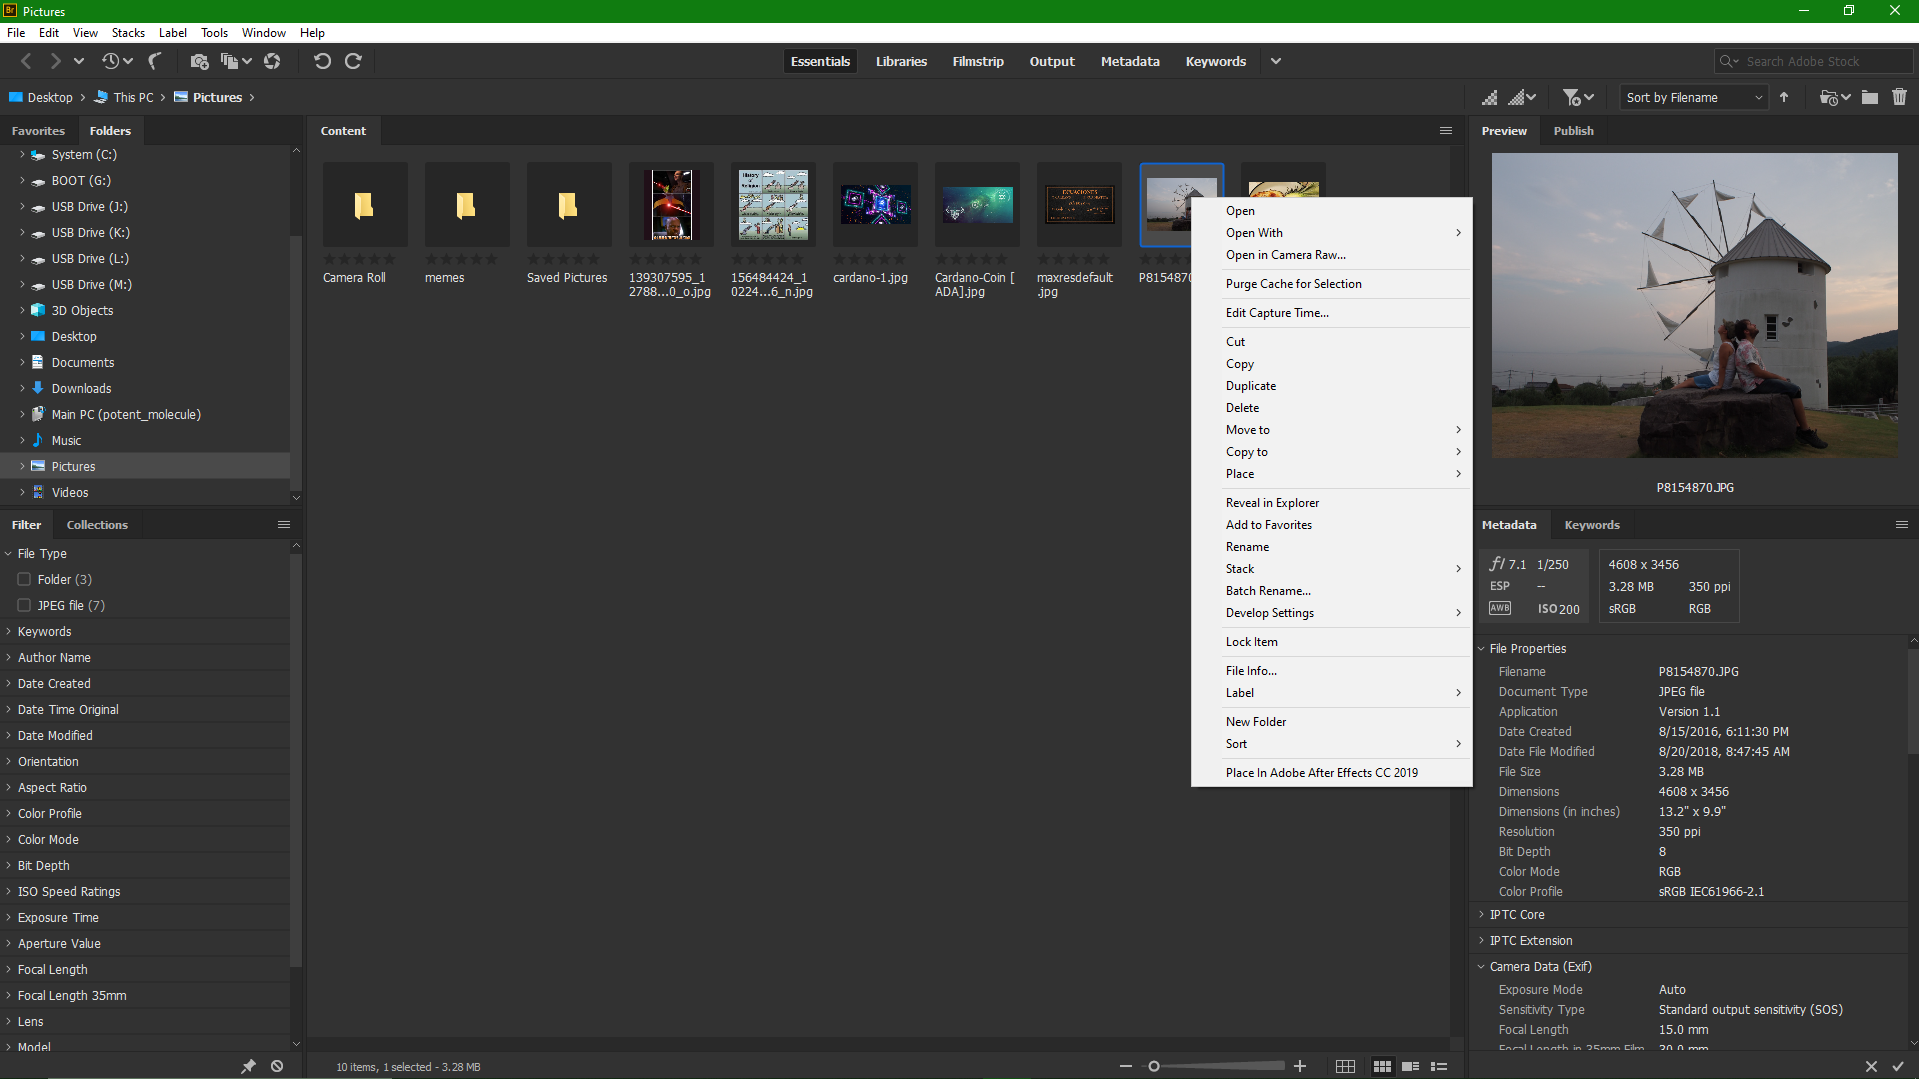
\includegraphics[width=0.7\textwidth]{images/bridge.png}
					\end{center}
				\end{frame}
	
	\begin{frame}
		\frametitle{Camera Raw}
		\begin{outline}
			\1 Camera Raw provides you with all of the same tools that are found in Photoshop.
			\1 But, It is just focused on "developing" images, rather than on "manipulating" them.
			\1 Thus you will find all the tools you need to manually correct and adjust an images colors.
			\1 Press the Q key to toggle before/after preview.
		\end{outline}
	\begin{center}
		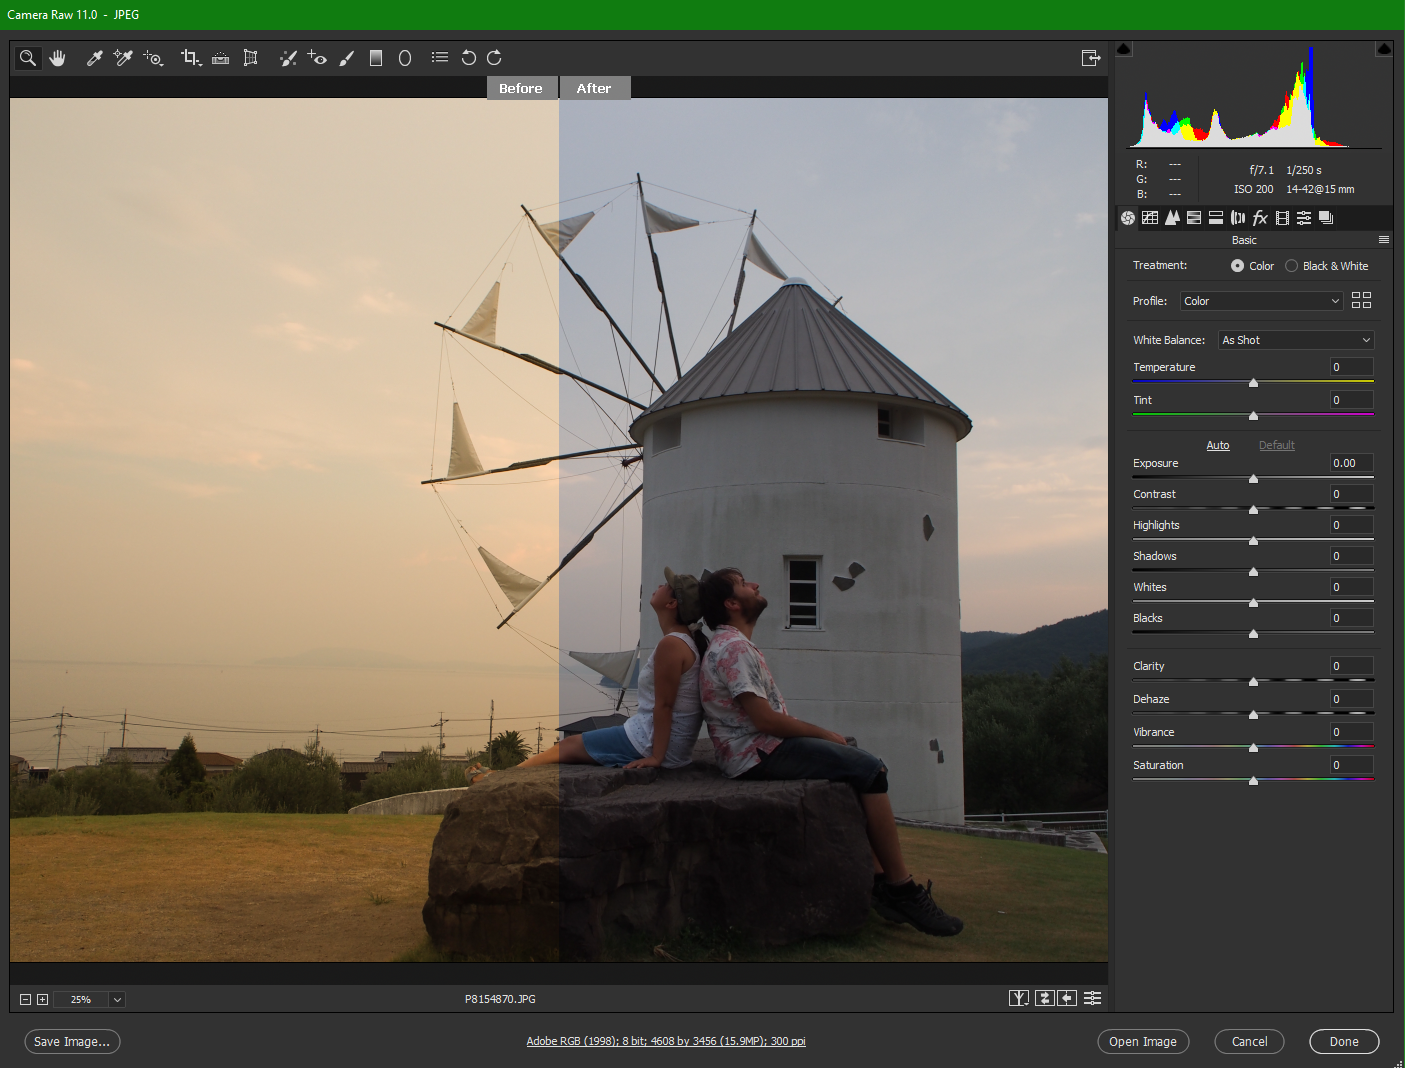
\includegraphics[width=0.55\textwidth]{images/camera raw.png}
	\end{center}
	\end{frame}	


\end{document}